\section{Local Deblur Sharpening protocol}
\label{app:localDeblurSharpening}%a101

Protocol designed to apply $LocalDeblur$, the automatic local resolution-based method that increases map signal at medium/high resolution \citep{ramirez2018}, in \scipion. Unlike similar approaches, $LocalDeblur$ does not need any prior atomic model, avoiding artificial structure factor corrections.

\begin{itemize}
 \item Requirements to run this protocol and visualize results:
    \begin{itemize}
        \item \scipion plugin: \ttt{scipion-em-xmipp}
    \end{itemize}
 \item \scipion menu:\\
  \ttt{Model building -> Preprocess map} (\ffigure{fig:app_localdeblur_1} (A))
  
 \item Protocol form parameters (\ffigure{fig:app_localdeblur_1} (B)):
  
    \begin{figure}[H]
     \centering 
     \captionsetup{width=.7\linewidth} 
     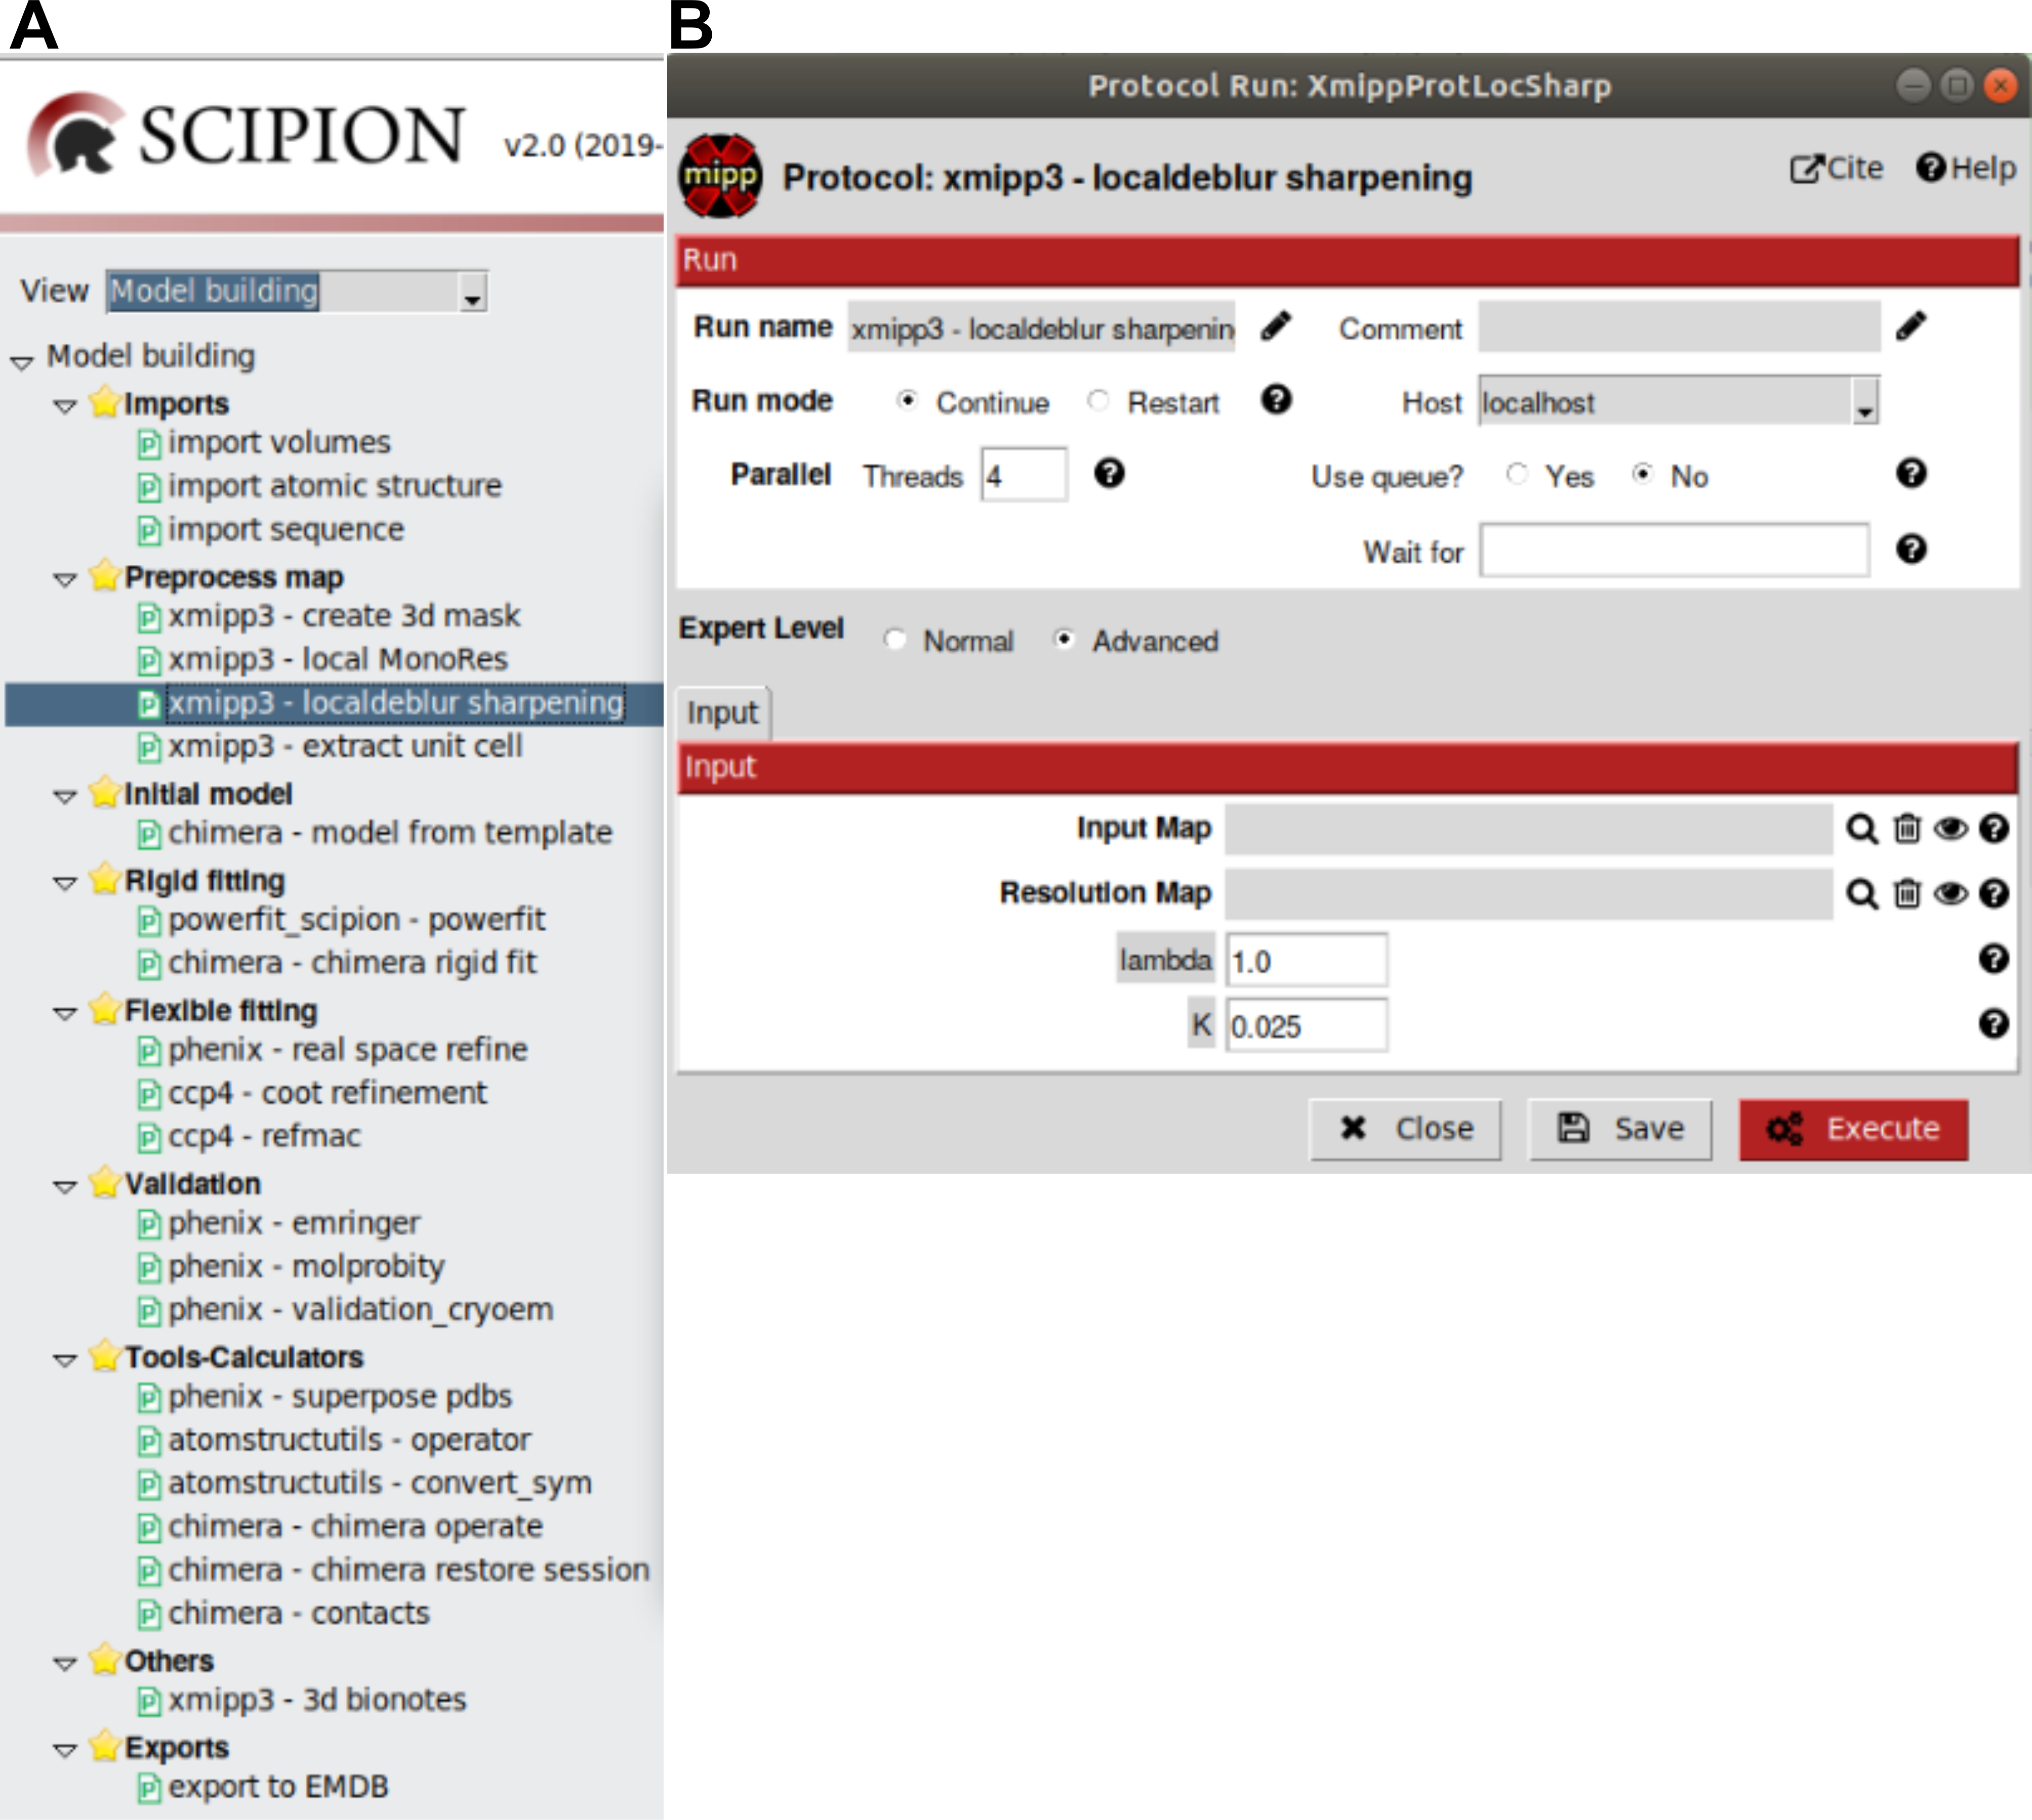
\includegraphics[width=0.90\textwidth]{Images_appendix/Fig208}
     \caption{Protocol \scommand{xmipp3 - localdeblur sharpening}. A: Protocol location in \scipion menu. B: Protocol form.}
     \label{fig:app_localdeblur_1}
    \end{figure}
    
    \begin{itemize}
        \item \ttt{Input map}: Unfiltered electron density map previously downloaded or generated in \scipion.
        \item \ttt{Resolution Map}: Resolution map generated by protocols like \scommand{xmipp3 - local MonoRes}. The resolution value in the corresponding voxel of the \ttt{Input map} is assigned to each voxel of the \ttt{Resolution Map}.
        \item \ttt{lambda}: Since $LocalDeblur$ is based on an iterative formula repeated until a convergence criterion is reached, \ttt{$lambda$} is the step size advanced parameter that modulates the speed of convergence. The default value, \ttt{$lambda$} = 1, indicates that the method itself establishes automatically the value of \ttt{$lambda$}. Although the default value is small enough to guarantee the convergence and large enough to speed it up, the \ttt{$lambda$} value can be increased by the user to accelerate the convergence process. Unlike the default value, that grows along the convergence process, the \ttt{$lambda$} value selected by the user will be maintained constant. Falling into a local minimum is a risk derived of increasing the convergence speed.
        \item \ttt{K}: Weight assigned to the difference between the local resolution and the spatial frequency of the center of each bandpass filter. This difference weighted by \ttt{K} is the base to compute the local weight of each channel in the filter bank, that correlates the input map with the sharpened map. The bigger the value of \ttt{K}, the lower the weight of each channel in the filter bank. Maximum weights are obtained when local resolution and spatial frequency of the center of each bandpass filter show identical values.
    \end{itemize}
    
    \item Protocol execution:\\
  Adding specific map/structure label is recommended in \ttt{Run name} section, at the form top. To add the label, open the protocol form, press the pencil symbol at the right side of \ttt{Run name} box, complete the label in the new opened window, press OK and, finally, close the protocol. This label will be shown in the output summary content (see below). If you want to run again this protocol, do not forget to set to \ttt{Restart} the \ttt{Run mode}.\\
  Press the \ttt{Execute} red button at the form bottom.
  
  \item Visualization of protocol results:
  
  After executing the protocol, press \ttt{Analyze Results} and a menu window will be opened with $ShowJ$ (\url{https://github.com/I2PC/scipion/wiki/ShowJ}), the default \scipion viewer, including the maps generated in each independent iteration before getting convergence. The sharpening algorithm stops when the difference between two successive iterations is lower than 1\%, thus generating variable number of maps before stopping. The $ShowJ$ window menu (\ttt{File -> Open with Chimera}) allows to open the selected map in $Chimera$ graphics window.
  
  \item Summary content:
  \begin{itemize}
     \item Protocol output (below \scipion framework):\\ \ttt{xmipp3 - localdeblur sharpening -> ouputVolumes}; SetOfVolumes (number of items, x, y, and z dimensions, sampling rate).
     \item \ttt{SUMMARY} box:\\ \ttt{LocalDeblur Map}.
  \end{itemize}
    
\end{itemize}
